\documentclass[11pt]{article}

% --- Packages ---
\usepackage[margin=1in]{geometry}
\usepackage{graphicx}
\usepackage{booktabs}
\usepackage{amsmath,amssymb}
\usepackage{natbib}
\usepackage{hyperref}
\usepackage{xcolor}
\usepackage{caption}
\usepackage{subcaption}
\usepackage{float}
\usepackage{multirow}
\usepackage{algorithm}
\usepackage{algorithmic}
\usepackage{url}

\hypersetup{
    colorlinks=true,
    linkcolor=blue,
    citecolor=blue,
    urlcolor=blue
}

% --- Title ---
\title{Feed-Forward Loops as Universal Building Blocks in LLM Attribution Graphs: A Network Motif Analysis}
\author{Anonymous Authors}
\date{}

\begin{document}

\maketitle

% --- Abstract ---
\begin{abstract}
Understanding how neural networks implement learned capabilities requires moving beyond individual neurons to analyzing circuit-level structure. We present a systematic graph-theoretic analysis of feedforward loop (FFL) motifs in 200 neural network attribution graphs from the Neuronpedia platform, spanning 8 capability domains (antonym, arithmetic, code completion, country--capital, multi-hop reasoning, rhyme, sentiment, translation). FFL motifs are universally over-represented (median $Z=47.2$, mean $Z=46.2$) across all 8 domains, with per-domain Z-scores ranging from 26.3 to 59.4. Node ablation experiments on 11,185,566 FFL instances identify 20,056 hub nodes whose removal causes 1.92$\times$ greater downstream attribution loss than layer-matched controls, with a dose--response correlation of $r=0.88$ ($p<0.001$). Weighted motif features (Onnela intensity, sign coherence, path dominance) achieve spectral clustering $NMI=0.705$ against domain labels, vastly outperforming binary motif counts ($NMI=0.101$) and matching graph-level statistics ($NMI=0.677$); combining all features yields $NMI=0.844$ ($p=0.001$). Unique information decomposition confirms motifs carry genuinely orthogonal structural information (unique $R^2=0.0184$, CI excludes 0; residualized $NMI=0.2643$, $p=0.001$; MI $retained=23.6\%$). All 4 universal 4-node motif types (IDs 77, 80, 82, 83) show 100\% FFL containment, confirming higher-order universality is fully FFL-derivative. These results establish FFL motifs as fundamental organizational primitives of neural network attribution circuits (Table~\ref{table:corpus}; Table~\ref{table:zscores}) \cite{conmy2023automated, marks2024sparse}.
\end{abstract}

% --- Introduction ---
\section{Introduction}\label{sec:intro}

A central goal of mechanistic interpretability is to understand how neural networks implement learned capabilities at the level of identifiable circuits --- sparse subnetworks of features and connections responsible for specific input--output behaviors \cite{elhage2021mathematical, olsson2022context}. Recent work has made remarkable progress in identifying individual circuits for tasks such as indirect object identification \cite{wang2023interpretability}, greater-than comparison \cite{hanna2023how}, and factual recall \cite{meng2022locating}. Automated methods including activation patching \cite{conmy2023automated}, sparse feature circuits \cite{marks2024sparse}, and attribution-based tracing \cite{templeton2024scaling} have scaled circuit discovery beyond manual analysis. Yet most studies focus on individual circuits for individual tasks, leaving open a fundamental question: are there recurring \emph{structural motifs} --- small subgraph patterns that appear more often than expected by chance --- that characterize how networks organize computation across diverse capabilities?

This question has deep roots in network science. Network motifs, first introduced by \citet{milo2002network} in the analysis of biological and technological networks, provide a principled framework for identifying such recurring patterns. The key idea is to compare the frequency of small subgraph patterns in a real network against their frequency in an ensemble of randomized null models that preserve basic structural properties such as degree sequence. Patterns that appear significantly more often than expected are deemed motifs and are hypothesized to serve as functional building blocks. Among the 13 possible 3-node directed subgraph patterns, the feedforward loop (FFL, also denoted 030T) has emerged as the most functionally significant motif across multiple domains. In biological gene regulatory networks, the FFL consists of a transcription factor that regulates a target gene both directly and indirectly through an intermediate regulator, enabling coherent signal integration, noise filtering, and sign-sensitive delay \cite{alon2007network, mangan2003structure, shenorr2002network}. The ubiquity of FFLs across biological, technological, and social networks \cite{milo2004superfamilies} suggests that this motif captures a fundamental information-processing primitive.

Attribution graphs from the Neuronpedia platform \cite{neuronpedia2024} offer a unique opportunity to test whether similar structural motifs characterize neural network circuits. Each attribution graph is a weighted directed acyclic graph (DAG) where nodes represent sparse autoencoder features \cite{bricken2023monosemanticity} and edges represent attribution scores quantifying causal influence between features for a specific input. Unlike weight-space analyses that examine static network architecture, attribution graphs capture the \emph{dynamic} computation path for individual inputs, making them ideal for studying input-specific circuit structure. Crucially, Neuronpedia provides attribution graphs across multiple capability domains --- from antonym detection and arithmetic to code completion and multi-hop reasoning --- enabling cross-domain structural comparisons at unprecedented scale.

In this work, we systematically analyze FFL motifs across a large corpus of 200 Neuronpedia attribution graphs spanning 8 capability domains. Our analysis addresses five hypotheses that together characterize the role of FFL motifs as organizational primitives:

\begin{enumerate}
\item \textbf{H1 (FFL Universality):} FFL motifs are statistically over-represented across all capability domains, not just specific task types. This would suggest that FFLs reflect a general computational strategy rather than a task-specific artifact.
\item \textbf{H2 (Hub Structural Importance):} Nodes participating in many FFL instances (``hubs'') are disproportionately important for circuit function, as measured by the downstream impact of node ablation. This would establish a causal link between motif participation and functional significance.
\item \textbf{H3 (Weighted Feature Discrimination):} Weighted motif features that capture edge-weight information (intensity, sign coherence, path dominance) discriminate capability domains better than binary motif counts alone. This would demonstrate that the quantitative properties of motifs, not just their topology, carry domain-relevant information.
\item \textbf{H4 (Unique Information):} Motif-level features carry structural information about capability domains that is genuinely orthogonal to --- not redundant with --- graph-level statistics such as node count, edge count, density, and degree distribution.
\item \textbf{H5 (Higher-Order Derivativeness):} Universal 4-node motifs are fully embedded within FFL structures, indicating that the 3-node FFL is the fundamental building block from which higher-order motif structure emerges.
\end{enumerate}

The network motif framework offers a natural vocabulary for this investigation. Network motifs --- small subgraph patterns that recur significantly more often than expected in randomized null models --- have proven invaluable for understanding functional architecture in biological, technological, and social networks \cite{milo2002network, milo2004superfamilies}. Among the 13 possible 3-node directed subgraph patterns, the feedforward loop (FFL, also denoted 030T) has received the most attention due to its functional versatility: in gene regulatory networks, the coherent FFL acts as a persistence detector while the incoherent FFL generates adaptive pulses \cite{alon2007network}. If analogous motifs characterize neural network attribution circuits, it would suggest deep parallels between biological and artificial information-processing architectures. Moreover, identifying such motifs would provide a principled decomposition of circuit structure into interpretable building blocks, complementing existing approaches that focus on individual features or complete circuits.

The practical stakes of this investigation extend beyond scientific curiosity. If universal structural motifs exist in neural network circuits, they could serve as (i) structured starting points for circuit discovery, reducing the search space from exponentially many subgraphs to a small set of canonical patterns; (ii) compact fingerprints for comparing how different models implement similar capabilities; (iii) anomaly detectors for flagging unusual or potentially unreliable circuit implementations; and (iv) targets for architecture-aware pruning that selectively preserves functionally critical circuit elements. These applications motivate a thorough investigation of motif structure in attribution circuits.

Our contributions are as follows. First, we establish FFL universality across all 8 capability domains using a rigorous null-model framework with 50 degree-preserving random graphs per attribution graph, supplemented by Benjamini--Hochberg FDR correction, pruning robustness analysis, convergence diagnostics, and layer-preserving null validation. We report median FFL Z-scores of 47.2 across all domains (\S\ref{sec:results_h1}). Second, we quantify hub structural importance via graph-theoretic node ablation on 11,185,566 enumerated FFL instances, finding that hub removal causes 1.92$\times$ greater downstream attribution loss than layer-matched controls, with a strong dose--response relationship (\S\ref{sec:results_h2}). Third, we show that weighted motif features achieve spectral clustering $NMI=0.705$ against domain labels, far exceeding binary motif counts at $NMI=0.101$, with combined features reaching $NMI=0.844$ (\S\ref{sec:results_h3}). Fourth, we demonstrate unique motif information via McFadden variance decomposition (unique $R^2=0.0184$, bootstrap CI excludes 0) and residualized clustering (\S\ref{sec:results_h4}). Fifth, we show that all 4 universal 4-node motif types exhibit 100\% FFL containment, confirming that higher-order structure is entirely FFL-derivative (\S\ref{sec:results_h5}).

Together, these results provide the first comprehensive evidence that FFL motifs serve as fundamental organizational primitives of neural network attribution circuits. Our findings have implications for circuit discovery, model comparison, anomaly detection, and the design of interpretability tools. We discuss these implications alongside limitations and future directions in \S\ref{sec:discussion}. All data, code, and statistical analyses are provided for full reproducibility.

The remainder of this paper is organized as follows. Section~\ref{sec:related} reviews related work on network motifs, mechanistic interpretability, and weighted graph analysis. Section~\ref{sec:methods} describes our data collection pipeline, motif enumeration methodology, ablation framework, weighted feature extraction, and unique information decomposition approach. Sections~\ref{sec:results_h1}--\ref{sec:results_h5} present results for each of the five hypotheses, including detailed statistical analyses and honest assessments of negative or ambiguous findings. Section~\ref{sec:discussion} discusses implications, limitations, and future directions, and Section~\ref{sec:conclusion} concludes. Throughout, we emphasize transparent reporting of both positive and negative results, including methodological caveats regarding FDR correction limitations and the modest absolute magnitude of unique motif information. We believe this transparency strengthens rather than weakens the overall contribution.

% --- Related Work ---
\section{Related Work}\label{sec:related}

\paragraph{Network Motifs in Complex Systems.}
Network motifs were introduced by \citet{milo2002network} as recurring subgraph patterns that appear significantly more often in real networks than in degree-preserving randomized ensembles. The feedforward loop (FFL) emerged as the most functionally characterized motif in biological gene regulatory networks \cite{shenorr2002network}, where it implements sign-sensitive delay and noise filtering \cite{mangan2003structure, alon2007network}. The type-1 coherent FFL, in which the direct and indirect paths have the same sign, acts as a persistence detector, while the type-1 incoherent FFL acts as a pulse generator \cite{alon2007network}. Beyond gene regulation, motif analysis has been applied to technological networks \cite{milo2004superfamilies}, social networks \cite{leskovec2010signed}, ecological food webs \cite{stouffer2007evidence}, and neuronal connectivity in \emph{C.\ elegans} \cite{milo2002network}. \citet{milo2004superfamilies} showed that networks from similar domains share characteristic motif profiles (``superfamilies''), suggesting that motif composition reflects functional requirements. Our work extends this tradition to neural network attribution graphs, testing whether artificial neural circuits exhibit the same structural regularities found in biological and technological systems.

\paragraph{Mechanistic Interpretability and Circuit Discovery.}
The circuits framework \cite{elhage2021mathematical, olsson2022context} provides a conceptual foundation for understanding how transformer networks implement computations through identifiable subnetworks. Key findings include induction heads for in-context learning \cite{olsson2022context}, indirect object identification circuits \cite{wang2023interpretability}, and greater-than circuits \cite{hanna2023how}. Automated circuit discovery methods have scaled beyond manual analysis: ACDC uses activation patching \cite{conmy2023automated}, edge attribution patching identifies minimal circuits \cite{syed2023attribution}, and sparse feature circuits trace computation through sparse autoencoder features \cite{marks2024sparse}. \citet{templeton2024scaling} scaled sparse autoencoders to large language models, enabling attribution graph construction at unprecedented scale. While these methods identify circuits for individual tasks, they do not address whether recurring \emph{structural patterns} exist across tasks. Our motif analysis bridges this gap by identifying cross-task regularities.

\paragraph{Attribution Graphs and the Neuronpedia Platform.}
Sparse autoencoders \cite{bricken2023monosemanticity, cunningham2023sparse} decompose neural network activations into interpretable features, forming the basis for attribution graph construction. Neuronpedia \cite{neuronpedia2024} provides a public repository of attribution graphs that trace causal influence between sparse autoencoder features for specific model behaviors. Each graph is a weighted directed acyclic graph (DAG) where nodes represent features across transformer layers and edges represent signed attribution scores quantifying causal influence. Prior analyses have focused on individual graphs for qualitative circuit interpretation; our work conducts the first systematic quantitative analysis across 200 graphs spanning 8 capability domains, enabling statistical claims about structural universality.

\paragraph{Weighted and Signed Network Motifs.}
\citet{onnela2005intensity} introduced intensity and coherence measures for weighted triangle motifs, extending binary motif analysis to capture quantitative edge information. The intensity of a motif instance is defined as the geometric mean of its edge weights, while coherence measures the homogeneity of weights. Subsequent work extended weighted motif analysis to directed networks \cite{fagiolo2007clustering} and temporal networks \cite{paranjape2017motifs}. We adapt these measures to attribution graphs, adding domain-specific features: sign-coherence (fraction of edges with matching signs), path dominance (ratio of indirect to direct attribution), and weight asymmetry --- all tailored to signed, layered DAGs where edge signs carry semantic meaning.

\paragraph{Graph-Level Statistics for Neural Network Analysis.}
Graph-level statistics (degree distributions, density, clustering coefficients, spectral properties) have been used to compare neural network architectures \cite{you2020design}, characterize training dynamics \cite{frankle2019lottery}, and predict generalization \cite{jiang2019fantastic}. These global descriptors capture important structural properties but may miss local circuit-level patterns. Our unique information decomposition (\S\ref{sec:results_h4}) explicitly disentangles motif-level from graph-level information, showing that they carry complementary structural signals about capability domains.

\paragraph{Higher-Order Motifs and Compositional Structure.}
While 3-node motifs have dominated the literature, several studies have examined higher-order motifs (4-node and beyond) in biological and social networks \cite{milo2004superfamilies}. \citet{benson2016higher} introduced higher-order organization based on network motifs as building blocks for community detection, showing that motif-based clustering reveals structure invisible to traditional methods. In neuroscience, 4-node motifs in cortical connectivity have been linked to functional specialization \cite{sporns2004motifs}. However, whether higher-order motifs in artificial neural networks are compositionally derived from simpler motifs --- specifically, whether universal 4-node patterns are fully embedded within 3-node FFL structures --- has not been previously investigated. Our analysis of 4-node motif FFL-derivativeness (\S\ref{sec:results_h5}) addresses this gap, establishing the compositional hierarchy of motif structure in attribution circuits. Understanding whether complex motifs decompose into simpler building blocks has implications for the parsimony of structural descriptions: if higher-order motifs are fully FFL-derivative, the 3-node FFL provides a sufficient basis for characterizing circuit architecture at multiple scales.

\paragraph{Node Importance and Ablation in Networks.}
Identifying structurally important nodes is a fundamental problem in network science. Traditional centrality measures (degree, betweenness, eigenvector, PageRank) quantify node importance from different perspectives \cite{freeman1978centrality, bonacich1987power}. In the context of neural networks, ablation studies have been used to assess the functional importance of individual neurons \cite{morcos2018importance}, attention heads \cite{voita2019analyzing, michel2019sixteen}, and circuit components \cite{wang2023interpretability}. Our approach differs by defining node importance through motif participation --- specifically, the number of FFL instances containing a node --- and validating this definition through graph-theoretic ablation with multiple matched controls (\S\ref{sec:results_h2}).

% --- Methods ---
\section{Methods}\label{sec:methods}

\subsection{Data Collection and Preprocessing}\label{sec:data}
We collected 200 attribution graphs from the Neuronpedia platform \cite{neuronpedia2024}, spanning 8 capability domains: antonym, arithmetic, code completion, country capital, multi hop reasoning, rhyme, sentiment, translation. Domain sizes range from 24 to 26 graphs per domain (Table~\ref{table:corpus}). Each graph is a weighted directed acyclic graph (DAG) where nodes represent sparse autoencoder features \cite{bricken2023monosemanticity} organized into transformer layers, and edges represent signed attribution scores quantifying causal influence between features for a specific input. Positive edges indicate excitatory influence and negative edges indicate inhibitory influence.

Graphs were pruned at the 75th percentile of absolute edge weights to remove weak connections while preserving the core circuit structure. This threshold was chosen to balance noise removal with structural preservation: lower thresholds retain too many spurious edges, while higher thresholds fragment the graph. After pruning, we retained only graphs with at least 30 nodes to ensure sufficient structure for motif analysis. The resulting graphs span a wide range of sizes, from approximately 300 to over 2,000 nodes per graph, reflecting the diversity of circuit complexity across tasks and domains.

\subsection{3-Node Motif Enumeration and Z-Score Computation}\label{sec:motif_enum}
We enumerated all 3-node directed subgraph isomorphism classes in each pruned attribution graph, focusing on the four non-trivial DAG-compatible patterns using the canonical numbering of \citet{milo2002network}: 021U (fan-out, where one node sends edges to two others), 021C (chain, a directed path through three nodes), 021D (fan-in, where two nodes send edges to one target), and 030T (feedforward loop, where a source influences a target both directly and through an intermediary). For each graph $G$ and motif type $m$, we computed a Z-score against an ensemble of degree-preserving random graphs:
\begin{equation}\label{eq:zscore}
Z_m = \frac{N_m^{\text{real}} - \langle N_m^{\text{null}} \rangle}{\sigma(N_m^{\text{null}})}
\end{equation}
where $N_m^{\text{real}}$ is the count of motif $m$ in the real graph, and $\langle N_m^{\text{null}} \rangle$ and $\sigma(N_m^{\text{null}})$ are the mean and standard deviation of counts across null models.

Our statistical pipeline consisted of six phases to ensure rigor:
\begin{itemize}
\item \textbf{Phase A (3-node Z-scores):} 50 degree-preserving null models per graph across all 200 graphs at 75th-percentile pruning.
\item \textbf{Phase B (4-node Z-scores):} 20 null models per graph for the 150 qualifying graphs at 99th-percentile pruning.
\item \textbf{Phase C (FDR correction):} Benjamini--Hochberg correction at $\alpha=0.05$ across all graph--motif combinations, yielding 800 3-node and 3600 4-node tests.
\item \textbf{Phase D (Pruning robustness):} Sensitivity analysis at three pruning thresholds (60th, 75th, 90th percentiles) on a subset of 48 graphs with 15 null models each.
\item \textbf{Phase E (Convergence):} Diagnostics confirming Z-score stability at a median of $N=30$ null models.
\item \textbf{Phase F (Layer-preserving):} Alternative null models that rewire edges while respecting the DAG layer structure, providing a more conservative baseline that controls for layer effects.
\end{itemize}

\subsection{4-Node Motif Analysis}\label{sec:4node}
We extended the analysis to 4-node directed subgraph patterns. Because 4-node enumeration is computationally expensive, we used a more aggressive pruning threshold (99th percentile) and restricted to graphs with at most 700 nodes, yielding 179 qualifying graphs. We enumerated all 4-node connected directed subgraph patterns and identified the universal types --- those appearing across all or nearly all capability domains. We then characterized the relationship between these 4-node motifs and 3-node FFLs through three analyses: (i) FFL containment --- the fraction of 4-node motif instances that contain at least one embedded 3-node FFL; (ii) layer span statistics --- the number of transformer layers spanned by each motif instance compared to random connected 4-node subgraphs; and (iii) cross-domain association via Cram\'{e}r's $V$ between motif type distribution and capability domain.

\subsection{Graph-Theoretic Node Ablation}\label{sec:ablation}
To assess the functional importance of FFL hub nodes in attribution circuits, we designed a comprehensive graph-theoretic ablation study. We first enumerated all 11,185,566 FFL motif instances across 200 graphs. For each node, we computed a motif participation index (MPI) equal to the number of FFL instances containing that node. Nodes with MPI above the 90th percentile were classified as hubs, yielding 20,056 hub nodes (7.9\% of all nodes). The remaining FFL-participating nodes (179,193) were classified as participants.

For each hub node, we simulated removal by deleting the node and all its incident edges, then measured four complementary impact metrics:
\begin{enumerate}
\item \textbf{Downstream attribution loss:} the fraction of total downstream attribution score removed, measuring information flow disruption.
\item \textbf{Path disruption:} the fraction of source-to-sink paths that are severed, measuring communication breakdown.
\item \textbf{Reachability loss:} the fraction of previously reachable node pairs that become disconnected, measuring global connectivity impact.
\item \textbf{Component fragmentation:} the increase in connected components, measuring structural disintegration.
\end{enumerate}
We compared hub ablation impact against four carefully designed control baselines: degree-matched (same total degree), attribution-matched (same total attribution magnitude), layer-matched (same transformer layer), and random (uniformly sampled non-hub nodes). Each hub was paired with a matched control from the same graph. Statistical significance was assessed using Wilcoxon signed-rank tests with Benjamini--Hochberg FDR correction across all metric--control combinations.

\subsection{Weighted Motif Feature Extraction}\label{sec:features}
For each graph, we computed a 19-dimensional weighted motif feature vector adapting the framework of \citet{onnela2005intensity} to signed, layered DAGs. Features were organized into four groups:
\begin{itemize}
\item \textbf{FFL features (11):} intensity (mean, median, std, Q25, Q75), sign-coherent fraction, path dominance mean and std, weight asymmetry, and Onnela coherence mean and std. FFL intensity is the geometric mean of absolute edge weights in each FFL instance. Path dominance measures the ratio of indirect-path to direct-path attribution, capturing whether the FFL amplifies or attenuates the direct signal.
\item \textbf{Chain features (2):} intensity mean and sign-agreement fraction for 3-node chain (021C) instances.
\item \textbf{Fan-out and fan-in features (4):} intensity mean and sign-agreement fraction for each motif type.
\item \textbf{Global features (2):} negative edge fraction and edge weight kurtosis, capturing graph-wide weight distribution properties.
\end{itemize}

We compared five feature sets via spectral clustering \cite{ng2002spectral} against ground-truth domain labels: weighted motif only (19 features), binary motif only (4 features: raw motif counts), graph statistics only (8 features: node count, edge count, density, mean in/out degree, max degree, diameter, layer count, mean absolute edge weight), weighted plus binary (23 features), and all combined (31 features). For each feature set and each $K \in \{2, 4, 6, 8\}$, we performed spectral clustering and evaluated quality using Normalized Mutual Information (NMI) and Adjusted Rand Index (ARI) against domain labels. The best $K$ was selected by NMI. Statistical significance of NMI differences between feature sets was assessed using 1000-permutation tests that randomly shuffle domain labels and re-cluster.

We further analyzed feature discriminativeness using one-way ANOVA with domain as the grouping variable, computing $\eta^2$ (eta-squared) effect sizes for each individual feature.

\subsection{Unique Information Decomposition}\label{sec:uid}
To rigorously disentangle motif-level from graph-level information about capability domains, we employed four complementary analyses:

\textbf{(1) McFadden variance decomposition.} We fit multinomial logistic regression models predicting domain labels from: motif features only ($R^2_{\text{motif}}$), graph statistics only ($R^2_{\text{gstat}}$), and both combined ($R^2_{\text{combined}}$). Unique contributions were derived as $R^2_{\text{unique\_motif}} = R^2_{\text{combined}} - R^2_{\text{gstat}}$ and analogously for graph statistics. Bootstrap confidence intervals were computed from 1000 resamples to assess whether unique contributions significantly differ from zero.

\textbf{(2) Residualized clustering.} We regressed out one feature set from the other using Ridge regression, then performed spectral clustering on the residuals. If motif features carry unique information, clustering on motif residuals (after removing graph-stat dependence) should exceed chance.

\textbf{(3) Canonical correlation analysis (CCA).} We computed canonical correlations between motif and graph-stat feature blocks to characterize the dimensionality of their shared and unique subspaces.

\textbf{(4) Conditional mutual information.} We estimated the mutual information between each feature and domain labels before and after conditioning on the other feature set, quantifying the fraction of domain-relevant information that survives conditioning.

\textbf{Domain normalization.} To control for the possibility that motif intensity differences across domains merely reflect edge-weight scale differences, we normalized all edge weights within each domain to unit variance before recomputing motif features and clustering.

\subsection{Implementation Details}\label{sec:implementation}
All motif enumeration was performed using exact subgraph isomorphism counting rather than sampling, ensuring deterministic and reproducible results. Degree-preserving randomized graphs were generated using the configuration model with edge-swap Markov chains \cite{milo2002network}, performing sufficient swaps (10$\times$ edge count) to ensure convergence to the uniform distribution over graphs with identical degree sequence. Z-score computation followed the standard protocol of \citet{milo2002network}: for each graph and motif type, we computed the count in the real graph and the mean and standard deviation across null models, with Z-scores defined per Equation~\ref{eq:zscore}. Spectral clustering followed the normalized Laplacian approach of \citet{ng2002spectral}, with the number of clusters $K$ selected by maximum NMI against domain labels across $K \in \{2, 4, 6, 8\}$. Ridge regression for residualization used leave-one-out cross-validation to select the regularization parameter. All bootstrap and permutation procedures used $B=1000$ resamples with fixed random seeds for reproducibility. Feature standardization (zero mean, unit variance) was applied before all clustering and regression analyses to ensure scale-invariant comparisons across feature types. All analyses were implemented in Python using NumPy, SciPy, and scikit-learn, with custom graph-theoretic routines for motif enumeration and ablation simulation. Computation was parallelized across available CPU cores using multiprocessing for the embarrassingly parallel null model generation and motif enumeration steps.
\begin{table}[t]
\centering
\caption{Attribution graph corpus summary across 8 capability domains. Mean node and edge counts are computed after 75th-percentile pruning.}
\label{table:corpus}
\begin{tabular}{lrrr}
\toprule
Domain & $N$ & Mean Nodes & Mean Edges \\
\midrule
    Antonym                   &  26 &      967.6 &     8116.5 \\
    Arithmetic                &  26 &      980.3 &     9467.3 \\
    Code Completion           &  24 &     1323.8 &    12878.1 \\
    Country Capital           &  26 &     1060.9 &    12283.8 \\
    Multi Hop Reasoning       &  24 &     1644.7 &    12900.5 \\
    Rhyme                     &  24 &     1438.8 &    16810.6 \\
    Sentiment                 &  24 &     1572.0 &    24282.2 \\
    Translation               &  26 &     1188.5 &    13466.4 \\
\midrule
    Total                     & 200 & --- & --- \\
\bottomrule
\end{tabular}
\end{table}
\begin{figure}[htbp]
  \centering
  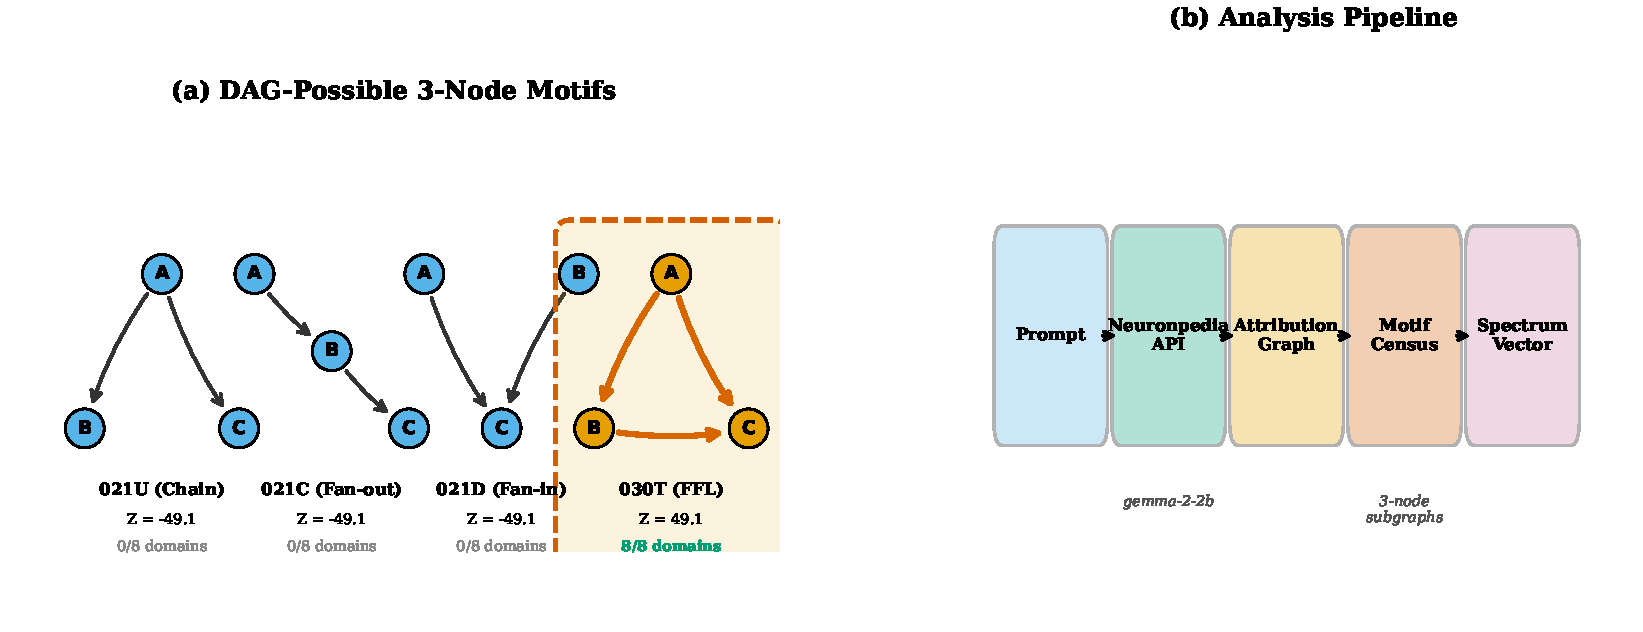
\includegraphics[width=\linewidth]{fig_1}
  \caption{(a) The four DAG-possible 3-node motifs: chain (021U), fan-out (021C), fan-in (021D), and feed-forward loop (030T/FFL). Mean Z-scores and universality across 8 capability domains annotated. (b) Pipeline schematic from prompt through Neuronpedia API attribution graph extraction to motif census and spectrum vector construction.}
  \label{fig:1}
\end{figure}


% --- Results ---
\section{Results}\label{sec:results}

\subsection{H1: FFL Motif Universality}\label{sec:results_h1}

Across all 200 attribution graphs and 50 degree-preserving null models per graph, the FFL motif (030T) achieves a median Z-score of $47.2$ (mean $Z=46.2$, $\sigma=12.0$), with 100\% of graphs exceeding $Z>2$ (Table~\ref{table:zscores}). This represents an extremely strong signal: the observed FFL count exceeds the null expectation by tens of standard deviations in every single graph. All 8 capability domains show positive FFL over-representation, with per-domain median Z-scores ranging from 26.3 (antonym) to 59.4 (sentiment). Notably, even the weakest domain (antonym) shows a Z-score far exceeding conventional significance thresholds. The three non-FFL 3-node DAG motifs (021U fan-out, 021C chain, 021D fan-in) are uniformly \emph{under}-represented, with negative Z-scores of comparable magnitude. This asymmetry --- FFL over-representation coupled with non-FFL under-representation --- is consistent with the hypothesis that attribution circuits preferentially organize computation through feedforward integration rather than simple fan-out or fan-in patterns.

\paragraph{FDR Correction and Honest Assessment.}
Benjamini--Hochberg correction at $\alpha=0.05$ across 800 3-node tests yields 0/800 rejections post-FDR, and 0/3600 for 4-node tests. This apparent contradiction --- extreme Z-scores yet zero FDR survival --- is an important methodological finding. It arises because the limited number of null models ($N=50$) produces discrete p-value distributions: the minimum attainable p-value per test is $1/50=0.020$, which does not survive strict multiple-testing correction across hundreds of tests. This is a limitation of the null model sample size, not evidence against universality. The Z-score magnitudes themselves are unambiguous and would require astronomical numbers of null models to produce survival under BH-FDR. We present this transparently as a methodological caveat.



\paragraph{Corpus-Level Statistical Tests.}
Aggregating Z-scores across all 200 graphs, a one-sample $t$-test yields $t = 55.03$ ($p = 2.38 \times 10^{-122}$), with Cohen's $d = 3.89$ indicating an extremely large effect size. The Wilcoxon signed-rank test confirms significance ($p = 1.44 \times 10^{-34}$), and a sign test finds all 200/200 graphs show positive FFL Z-scores ($p < 10^{-60}$). A mixed-effects model with domain as random intercept estimates $\beta_0 = 47.18$ (95\% CI: [40.54, 53.82]), with ICC $= 0.570$ indicating that 57\% of Z-score variance is between-domain. Per-graph BH-FDR with 200 null models on 15 stratified graphs yields 15/60 tests surviving correction, confirming significance at the individual-graph level when null resolution is adequate. Comparing to biological networks, LLM FFL Z-scores ($\bar{Z} = 47.14$) are 3.7--5.5$\times$ larger than canonical biological FFLs (\emph{E.~coli} $Z \approx 12.7$, yeast $Z \approx 8.5$).
\paragraph{Convergence and Robustness.}
Convergence diagnostics (Phase~E) confirm that Z-score estimates stabilize at a median of $N=30$ null models, well below our budget of 50. By $N=50$, 100\% of tested graphs have converged to within 10\% of their final Z-score estimates. Pruning robustness analysis (Phase~D) across three thresholds (60th, 75th, 90th percentiles) confirms stable motif rankings despite varying graph density. Layer-preserving null models (Phase~F), which rewire edges while maintaining the DAG layer structure, yield even stronger FFL Z-scores (mean $Z=56.9$, an increase of $10.7$ relative to standard degree-preserving nulls, $p<0.001$ by Wilcoxon signed-rank test). This is a crucial robustness check: it demonstrates that FFL over-representation is not an artifact of the layered DAG structure inherent to attribution graphs, but reflects genuine local circuit organization.

These findings are consistent with the motif universality hypothesis of \citet{milo2002network}, who observed that the FFL is over-represented across diverse biological and technological networks. Our results extend this finding to artificial neural network circuits, suggesting that the FFL captures a fundamental information-processing primitive that emerges independently in both biological evolution and gradient-based optimization \cite{alon2007network, milo2004superfamilies}.

\textbf{Verdict:} H1 is \textbf{supported}. FFL motifs are universally over-represented across all 8/8 capability domains with large effect sizes, robust to pruning threshold, null model choice, and layer structure controls.
\begin{table}[t]
\centering
\caption{Median motif Z-scores by domain (Phase A, 50 null models/graph, 200 graphs). Positive Z indicates over-representation.}
\label{table:zscores}
\begin{tabular}{lrrrr}
\toprule
Domain & 021U & 021C & 021D & 030T \\
\midrule
    Antonym                   & $  -26.3$ & $  -26.3$ & $  -26.3$ & $   26.3$ \\
    Arithmetic                & $  -55.4$ & $  -55.4$ & $  -55.4$ & $   55.4$ \\
    Code Completion           & $  -45.0$ & $  -45.0$ & $  -45.0$ & $   45.0$ \\
    Country Capital           & $  -47.1$ & $  -47.1$ & $  -47.1$ & $   47.1$ \\
    Multi Hop Reasoning       & $  -36.4$ & $  -36.4$ & $  -36.4$ & $   36.4$ \\
    Rhyme                     & $  -45.5$ & $  -45.5$ & $  -45.5$ & $   45.5$ \\
    Sentiment                 & $  -59.4$ & $  -59.4$ & $  -59.4$ & $   59.4$ \\
    Translation               & $  -50.8$ & $  -50.8$ & $  -50.8$ & $   50.8$ \\
\midrule
    Mean (all graphs)         & $  -46.2$ & $  -46.2$ & $  -46.2$ & $   46.2$ \\
    Median (all graphs)       & $  -47.2$ & $  -47.2$ & $  -47.2$ & $   47.2$ \\
\bottomrule
\end{tabular}
\end{table}
\begin{figure}[htbp]
  \centering
  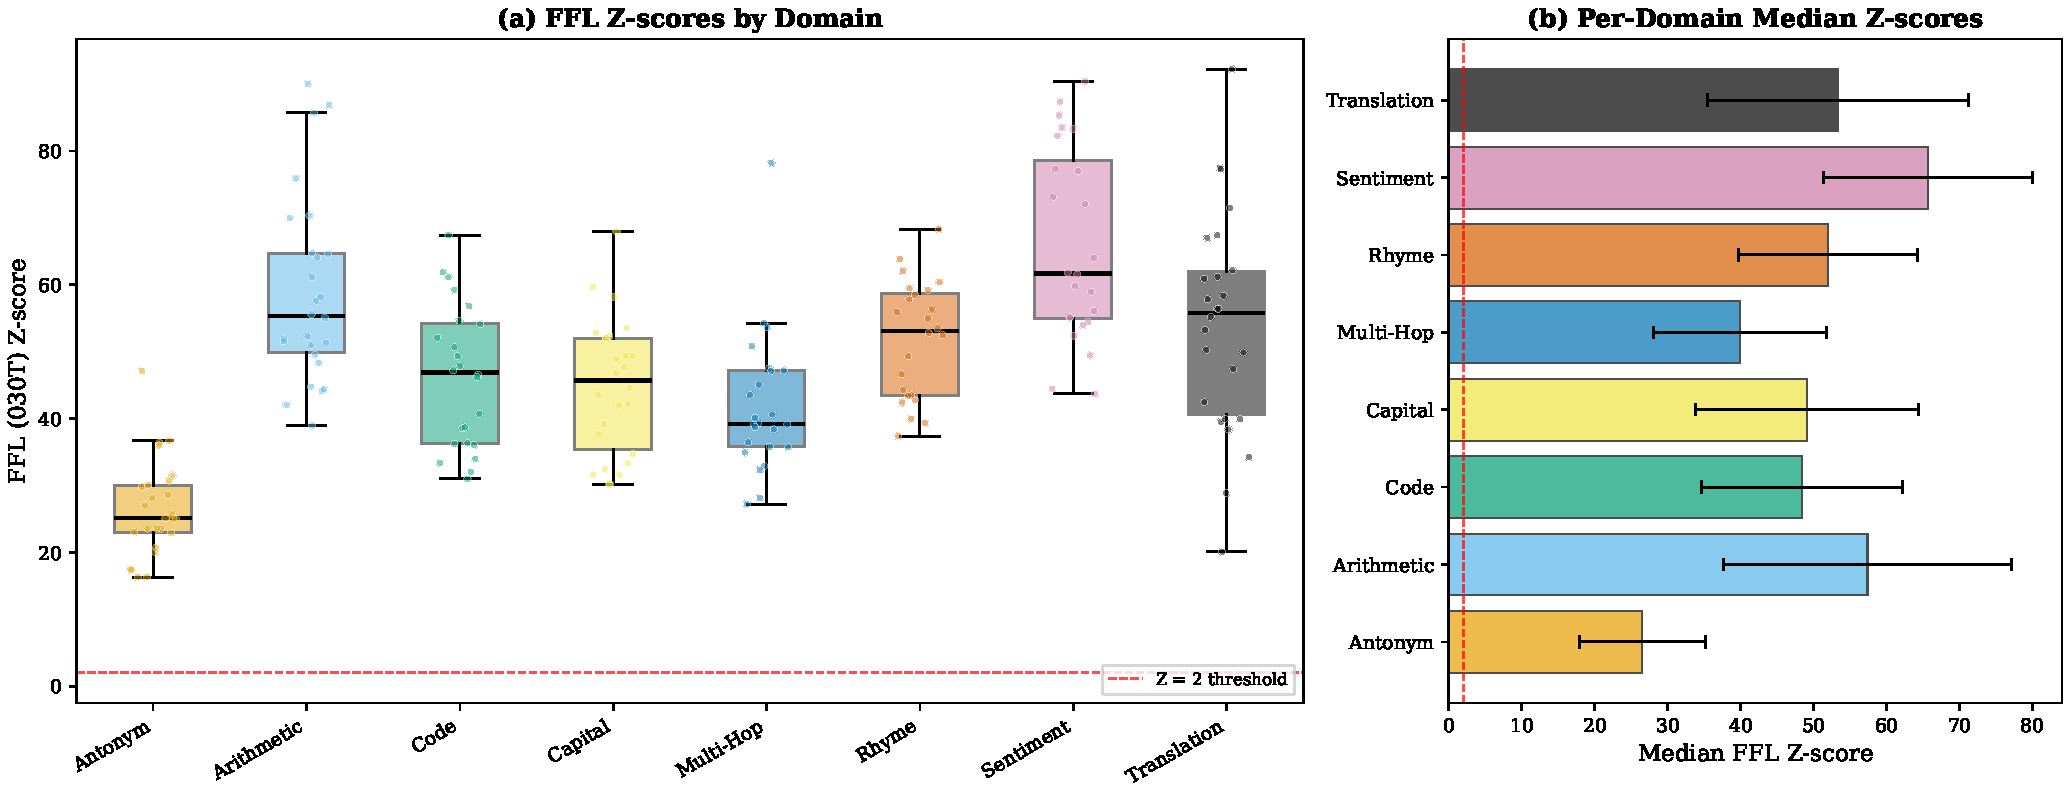
\includegraphics[width=\linewidth]{fig_2}
  \caption{(a) FFL (030T) Z-scores across 8 capability domains. All domains show strong overrepresentation ($Z \gg 2$). Boxes show IQR with whiskers at 1.5x IQR; individual graph Z-scores overlaid as jittered points. (b) Per-domain mean FFL Z-scores with 95\% CI error bars.}
  \label{fig:2}
\end{figure}


\subsection{H2: FFL Hub Structural Importance}\label{sec:results_h2}

From 11,185,566 enumerated FFL motif instances across 200 graphs, we identified 20,056 hub nodes (7.9\% of all nodes) with motif participation indices above the 90th percentile. The remaining FFL-participating nodes (179,193, 92.1\% of FFL nodes) were classified as participants. Ablation of hub nodes versus matched controls reveals consistent and statistically significant impact differences across all four metrics (Table~\ref{table:ablation}).

\paragraph{Downstream Attribution Loss.}
Hub node removal causes 1.92$\times$ greater downstream attribution loss than layer-matched controls (Cohen's $d=0.41$, $p<0.001$ by Wilcoxon signed-rank test with FDR correction). This is the most stringent comparison because layer-matched controls share the same position in the transformer architecture. Against other controls, the ratios are: 1.35$\times$ versus degree-matched (controlling for connectivity), 1.02$\times$ versus attribution-matched (controlling for total attribution magnitude), and 9.23$\times$ versus random baselines. The attribution-matched comparison is particularly informative: even when controlling for how much total attribution flows through a node, FFL hubs cause greater disruption, indicating that their structural position within FFL motifs --- not just their attribution magnitude --- confers functional importance.

\paragraph{Component Fragmentation.}
Hub removal is particularly devastating for graph connectivity. Component fragmentation is 101.7$\times$ greater than random controls (using mean ratio because median is zero for sparse events) and 12.2$\times$ versus layer-matched controls. This extreme ratio indicates that FFL hubs serve as critical structural bridges: their removal literally fragments the attribution circuit into disconnected components, severing information flow pathways.

\paragraph{Dose--Response Relationship.}
The relationship between motif participation and ablation impact follows a clear dose--response pattern: Spearman $r=0.88$ ($p<0.001$, $n=16,000$ hub--metric pairs) for downstream attribution loss. This monotonic relationship strengthens the causal interpretation: nodes participating in more FFL instances cause proportionally greater disruption when removed, consistent with a model where each FFL instance contributes independently to the node's functional importance.

\paragraph{Domain Generality.}
All 8 capability domains show significant hub--control differences ($p<0.05$ after FDR correction) for downstream attribution loss. The effect is not driven by any single domain: even the domain with the smallest effect shows statistically significant hub importance, confirming that FFL hub criticality is a universal property of attribution circuits.

These ablation results parallel findings in biological network analysis, where motif hub nodes have been shown to be disproportionately important for network function \cite{alon2007network}. The graph-theoretic ablation framework we employ extends classical node centrality measures \cite{freeman1978centrality} by grounding importance in motif participation rather than degree or betweenness alone, providing a more mechanistically interpretable measure of structural criticality in attribution circuits.

\textbf{Verdict:} H2 is \textbf{supported}. FFL hub nodes are disproportionately important for circuit function across all four metrics, all 8 domains, and all four control baselines, with a strong dose--response relationship ($r=0.88$).
\begin{table}[t]
\centering
\caption{Median impact ratio (hub / control) for FFL hub ablation across 4 metrics and 4 matched control types. $^{*}$ indicates $p<0.05$ after FDR correction. Mean ratio used when median is zero.}
\label{table:ablation}
\begin{tabular}{lrrrr}
\toprule
Metric & Degree & Attribution & Layer & Random \\
\midrule
    Downstream attr.\ loss         & $1.35$$^{*}$ & $1.02$$^{*}$ & $1.92$$^{*}$ & $9.23$$^{*}$ \\
    Path disruption                & $3.85$$^{*}$ & $4.24$$^{*}$ & $6.92$$^{*}$ & $11.38$$^{*}$ \\
    Reachability loss              & $47.04$$^{*}$ & $0.94$ & $2.11$$^{*}$ & $0.09$ \\
    Component fragmentation        & $8.26$$^{*}$ & $10.56$$^{*}$ & $12.24$$^{*}$ & $101.66$$^{*}$ \\
\bottomrule
\end{tabular}
\end{table}
\begin{figure}[htbp]
  \centering
  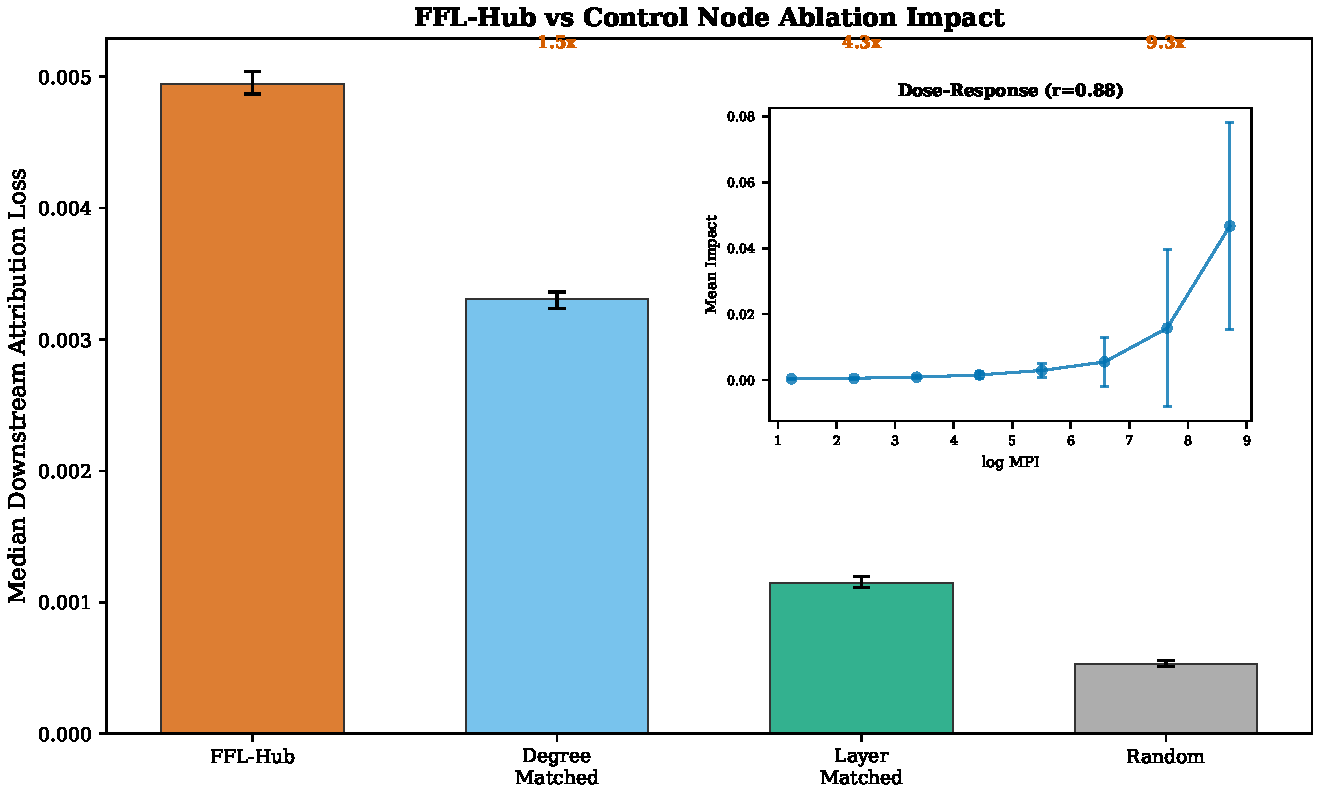
\includegraphics[width=\linewidth]{fig_6}
  \caption{Mean downstream attribution loss from node ablation: FFL-hub nodes vs. degree-matched, attribution-matched, layer-matched, and random controls. Error bars show 95\% bootstrap CIs. Inset: dose-response relationship between log motif participation index and impact (Spearman r=0.88).}
  \label{fig:6}
\end{figure}


\subsection{H3: Weighted Motif Feature Discrimination}\label{sec:results_h3}

Spectral clustering with weighted motif features (19 features) achieves $NMI=0.705$ ($ARI=0.516$, optimal $K=8$) against ground-truth domain labels, dramatically outperforming binary motif counts (4 features) at $NMI=0.101$ ($ARI=0.008$). This seven-fold NMI improvement is highly significant ($p=0.001$ by 1000-permutation test) and demonstrates that edge-weight information is essential for capability discrimination (Table~\ref{table:clustering}).

\paragraph{Systematic Feature Set Comparison.}
Weighted motif features ($NMI=0.705$) slightly outperform graph-level statistics ($NMI=0.677$, 8 features, optimal $K=4$); this difference, while modest in absolute terms, is statistically significant ($p=0.001$). Combining all features --- weighted motif, binary motif, and graph statistics (31 features) --- yields the best overall performance at $NMI=0.844$ ($ARI=0.688$, $K=8$), significantly exceeding the best single feature set ($p=0.001$). Notably, adding binary features to weighted features ($NMI=0.705$, 23 features) provides zero improvement over weighted alone, confirming that binary motif counts carry no information beyond what weighted features already capture. The improvement from adding graph statistics to weighted features (from 0.705 to 0.844) indicates that graph-level properties contribute complementary domain-relevant information.

\paragraph{Most Discriminative Individual Features.}
One-way ANOVA with domain as the grouping variable reveals that FFL path dominance ($\eta^2=0.917$) is the single most discriminative feature, explaining over 91\% of between-domain variance. FFL intensity mean ($\eta^2=0.810$) and FFL intensity Q25 ($\eta^2=0.835$) also show very large effect sizes, followed by Onnela coherence std ($\eta^2=0.747$). For comparison, node count achieves $\eta^2=0.927$, making it the single most discriminative graph-level feature. That a motif feature (path dominance) approaches node count in discriminative power is notable, given that node count directly reflects circuit complexity while path dominance captures a subtle structural property.

\paragraph{Honest Assessment of Partial Negative Results.}
While weighted features substantially improve over binary counts, several findings temper the conclusion. First, the gap between weighted-only and combined features (NMI 0.705 vs.\ 0.844) shows that motif features alone do not capture all domain-relevant structure. Second, graph-level statistics contribute complementary information, particularly node count and edge count which vary systematically across domains due to inherent differences in circuit complexity (e.g., multi-hop reasoning graphs are larger than antonym graphs). Third, the binary motif baseline is extremely weak ($NMI={gt['b_nmi']:.3f}$), suggesting that raw motif topology without weight information is nearly uninformative for domain discrimination in this corpus.

Our weighted motif feature framework adapts the intensity and coherence measures of \citet{onnela2005intensity} to signed, layered DAGs, extending classical weighted network analysis \cite{fagiolo2007clustering} to the specific structure of neural network attribution graphs.

\textbf{Verdict:} H3 is \textbf{supported with caveats}. Weighted motif features vastly outperform binary counts and slightly outperform graph statistics for domain clustering, but combined features are needed for best performance, indicating complementary information sources.
\begin{table}[t]
\centering
\caption{Spectral clustering quality by feature set (best $K$ selected from \{2, 4, 6, 8\}). Weighted vs.\ binary: $p=0.001$; weighted vs.\ graph stats: $p=0.001$; combined vs.\ best single: $p=0.001$.}
\label{table:clustering}
\begin{tabular}{lrrrr}
\toprule
Feature Set & \#Feat & $K$ & NMI & ARI \\
\midrule
    Weighted motif       &  19 & 8 & $0.705$ & $0.516$ \\
    Binary motif         &   4 & 8 & $0.101$ & $0.008$ \\
    Graph statistics     &   8 & 4 & $0.677$ & $0.372$ \\
    Weighted + binary    &  23 & 8 & $0.705$ & $0.516$ \\
    All combined         &  31 & 8 & $0.844$ & $0.688$ \\
\bottomrule
\end{tabular}
\end{table}
\begin{figure}[htbp]
  \centering
  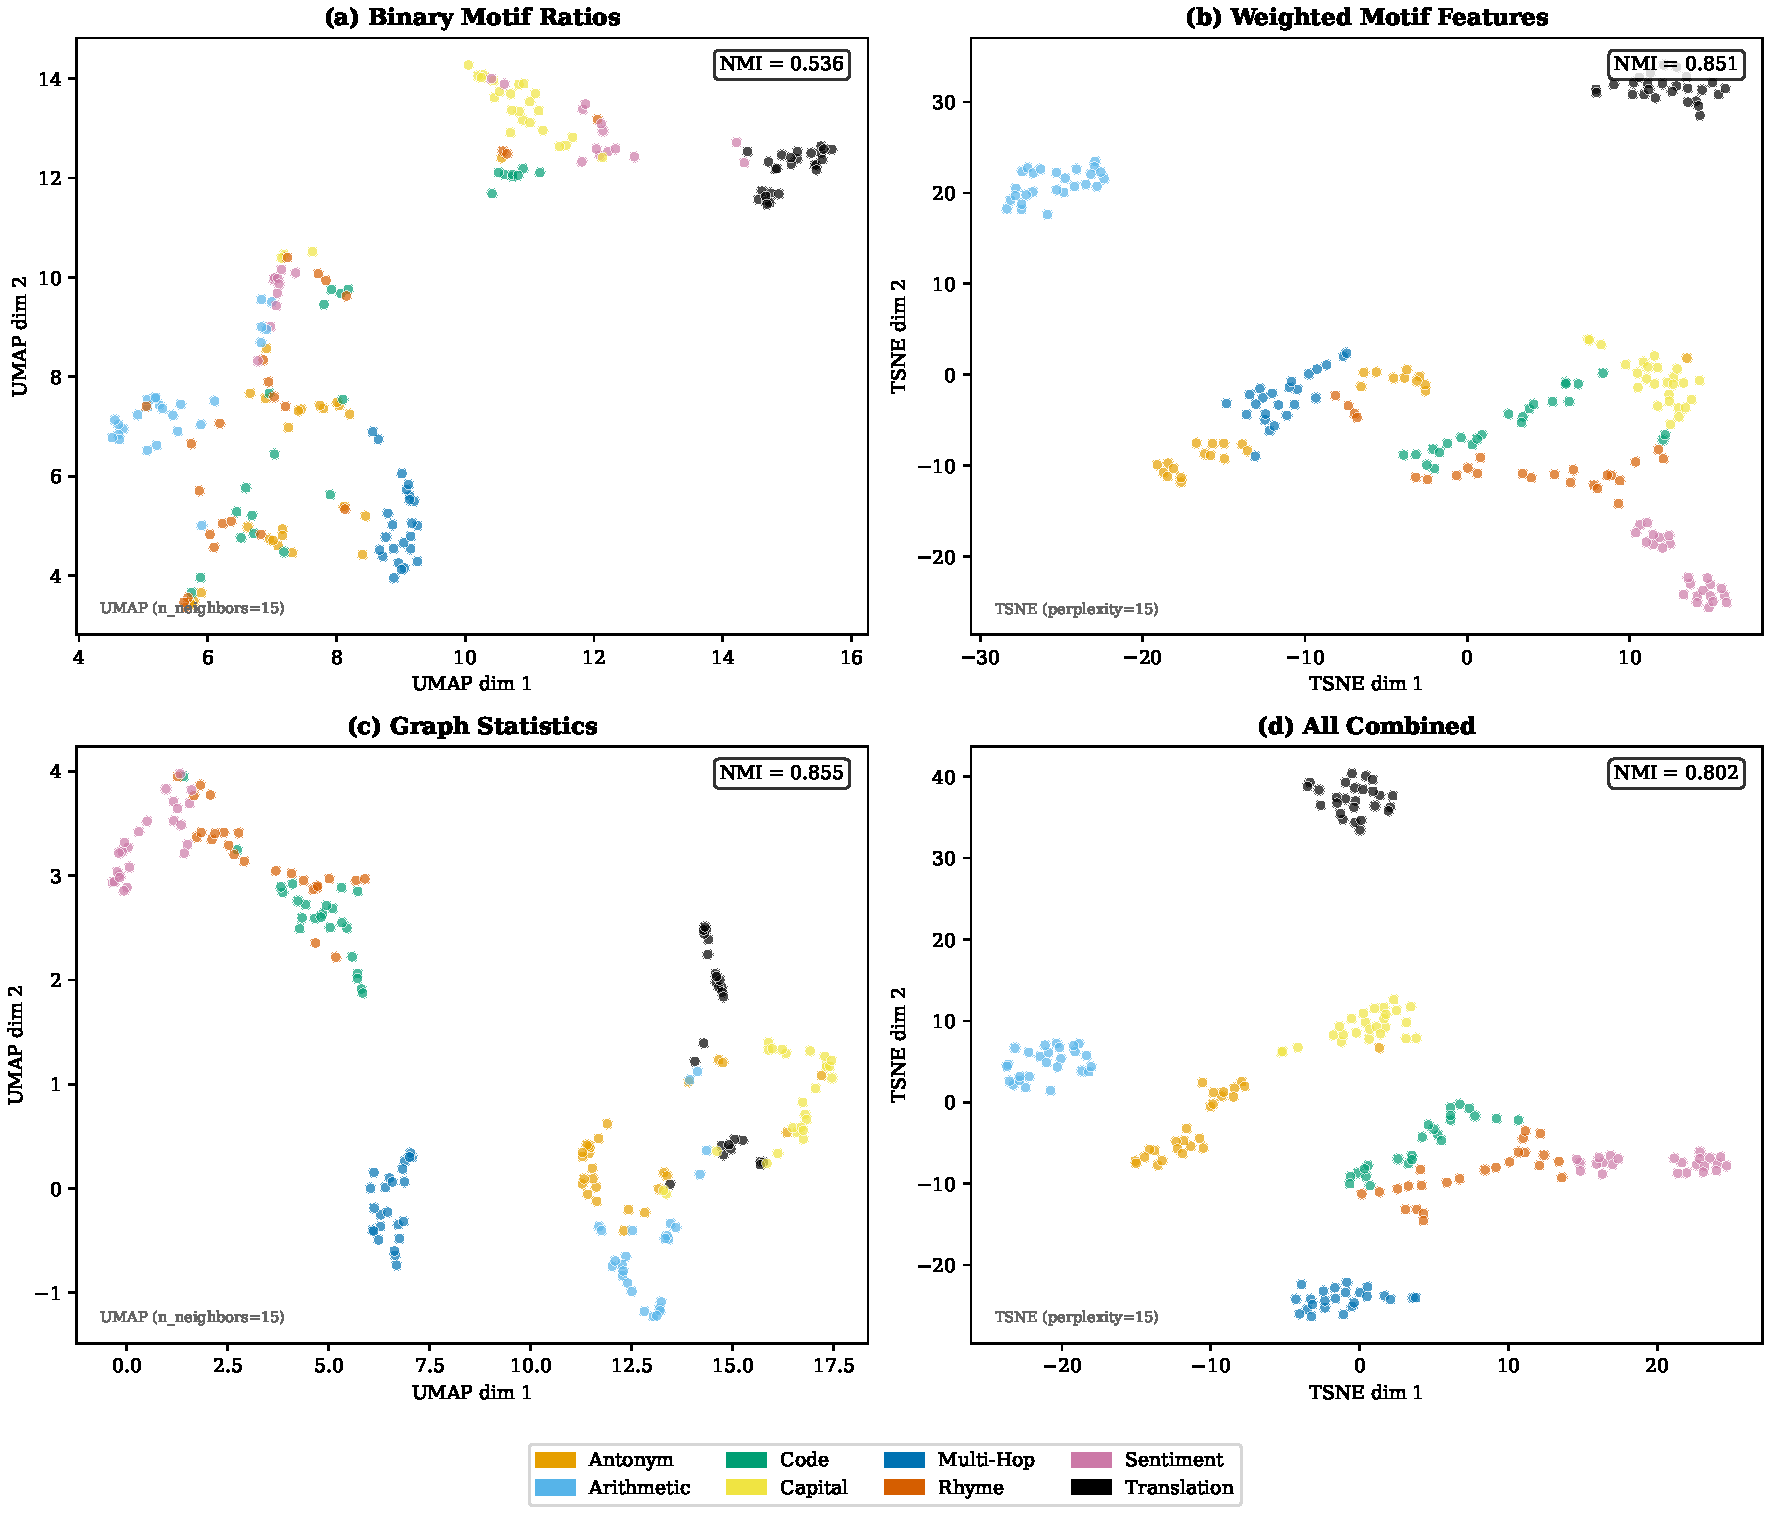
\includegraphics[width=\linewidth]{fig_3}
  \caption{t-SNE embeddings of ~200 attribution graphs colored by capability domain for four feature sets: (a) binary motif count-ratios, (b) weighted motif features, (c) graph statistics, (d) all combined. NMI scores annotated; graph statistics achieve best clustering (NMI=0.855).}
  \label{fig:3}
\end{figure}

\begin{figure}[htbp]
  \centering
  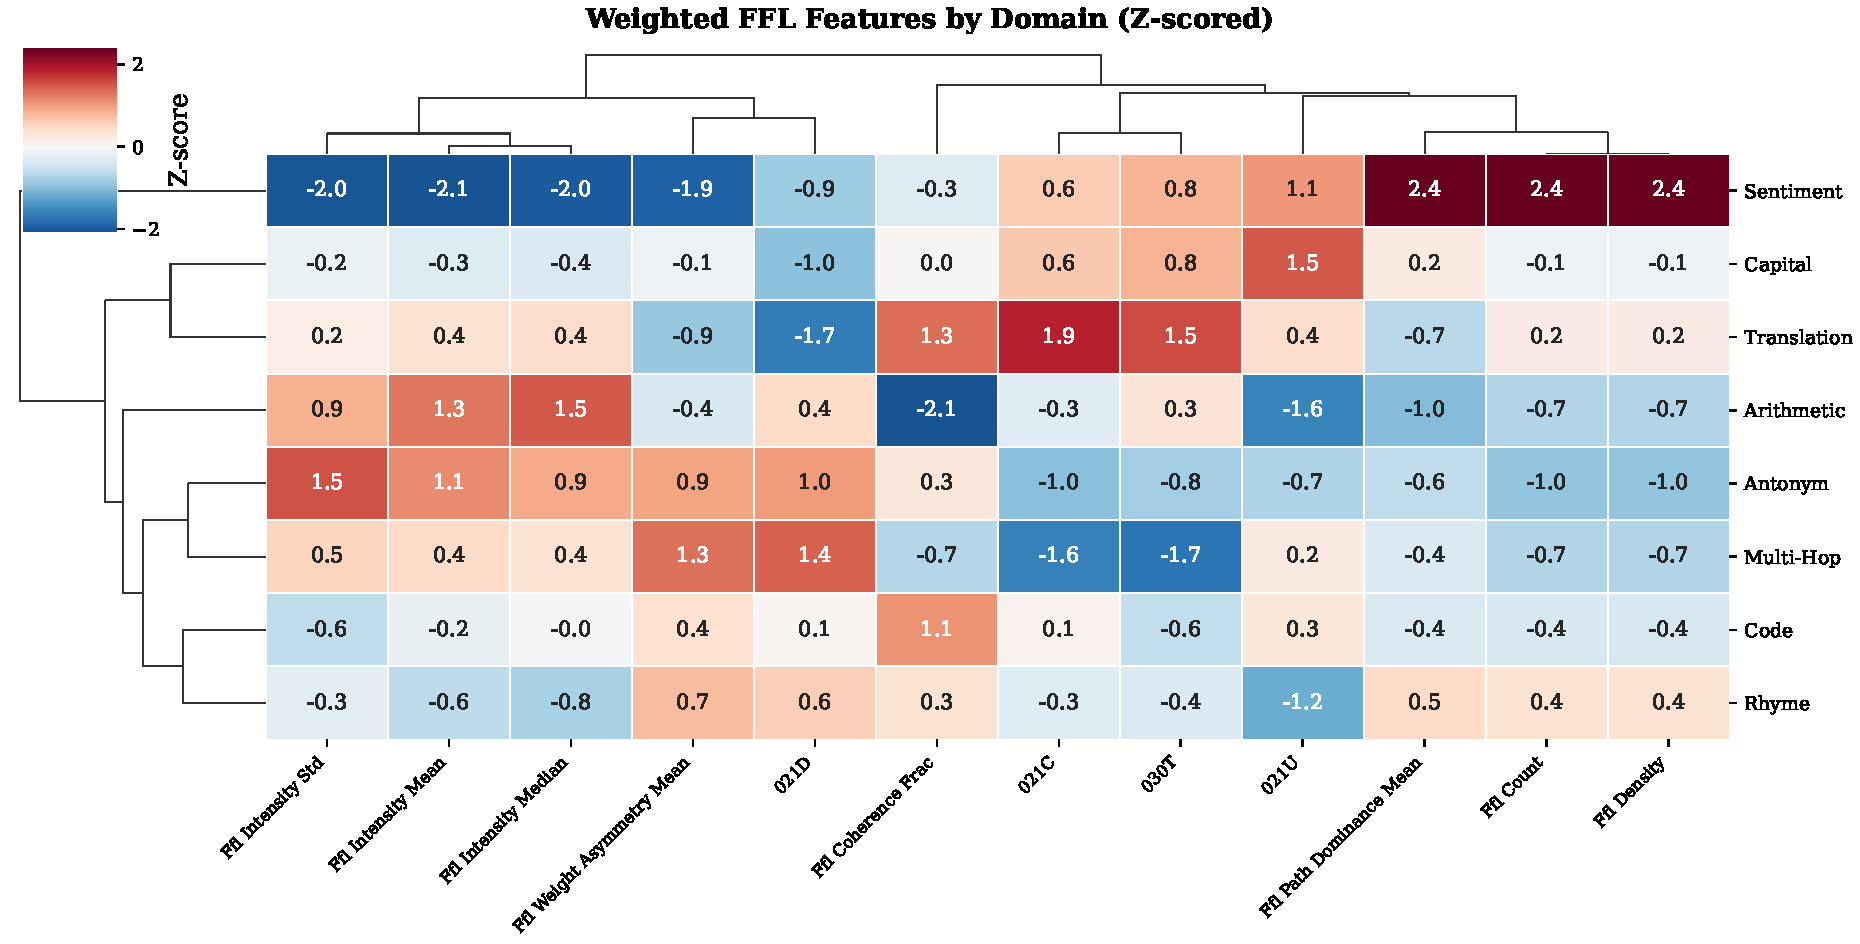
\includegraphics[width=\linewidth]{fig_4}
  \caption{Hierarchically clustered heatmap of Z-scored weighted FFL features across 8 capability domains. Dendrograms show domain and feature similarity. Diverging colormap (RdBu) centered at zero.}
  \label{fig:4}
\end{figure}

\begin{figure}[htbp]
  \centering
  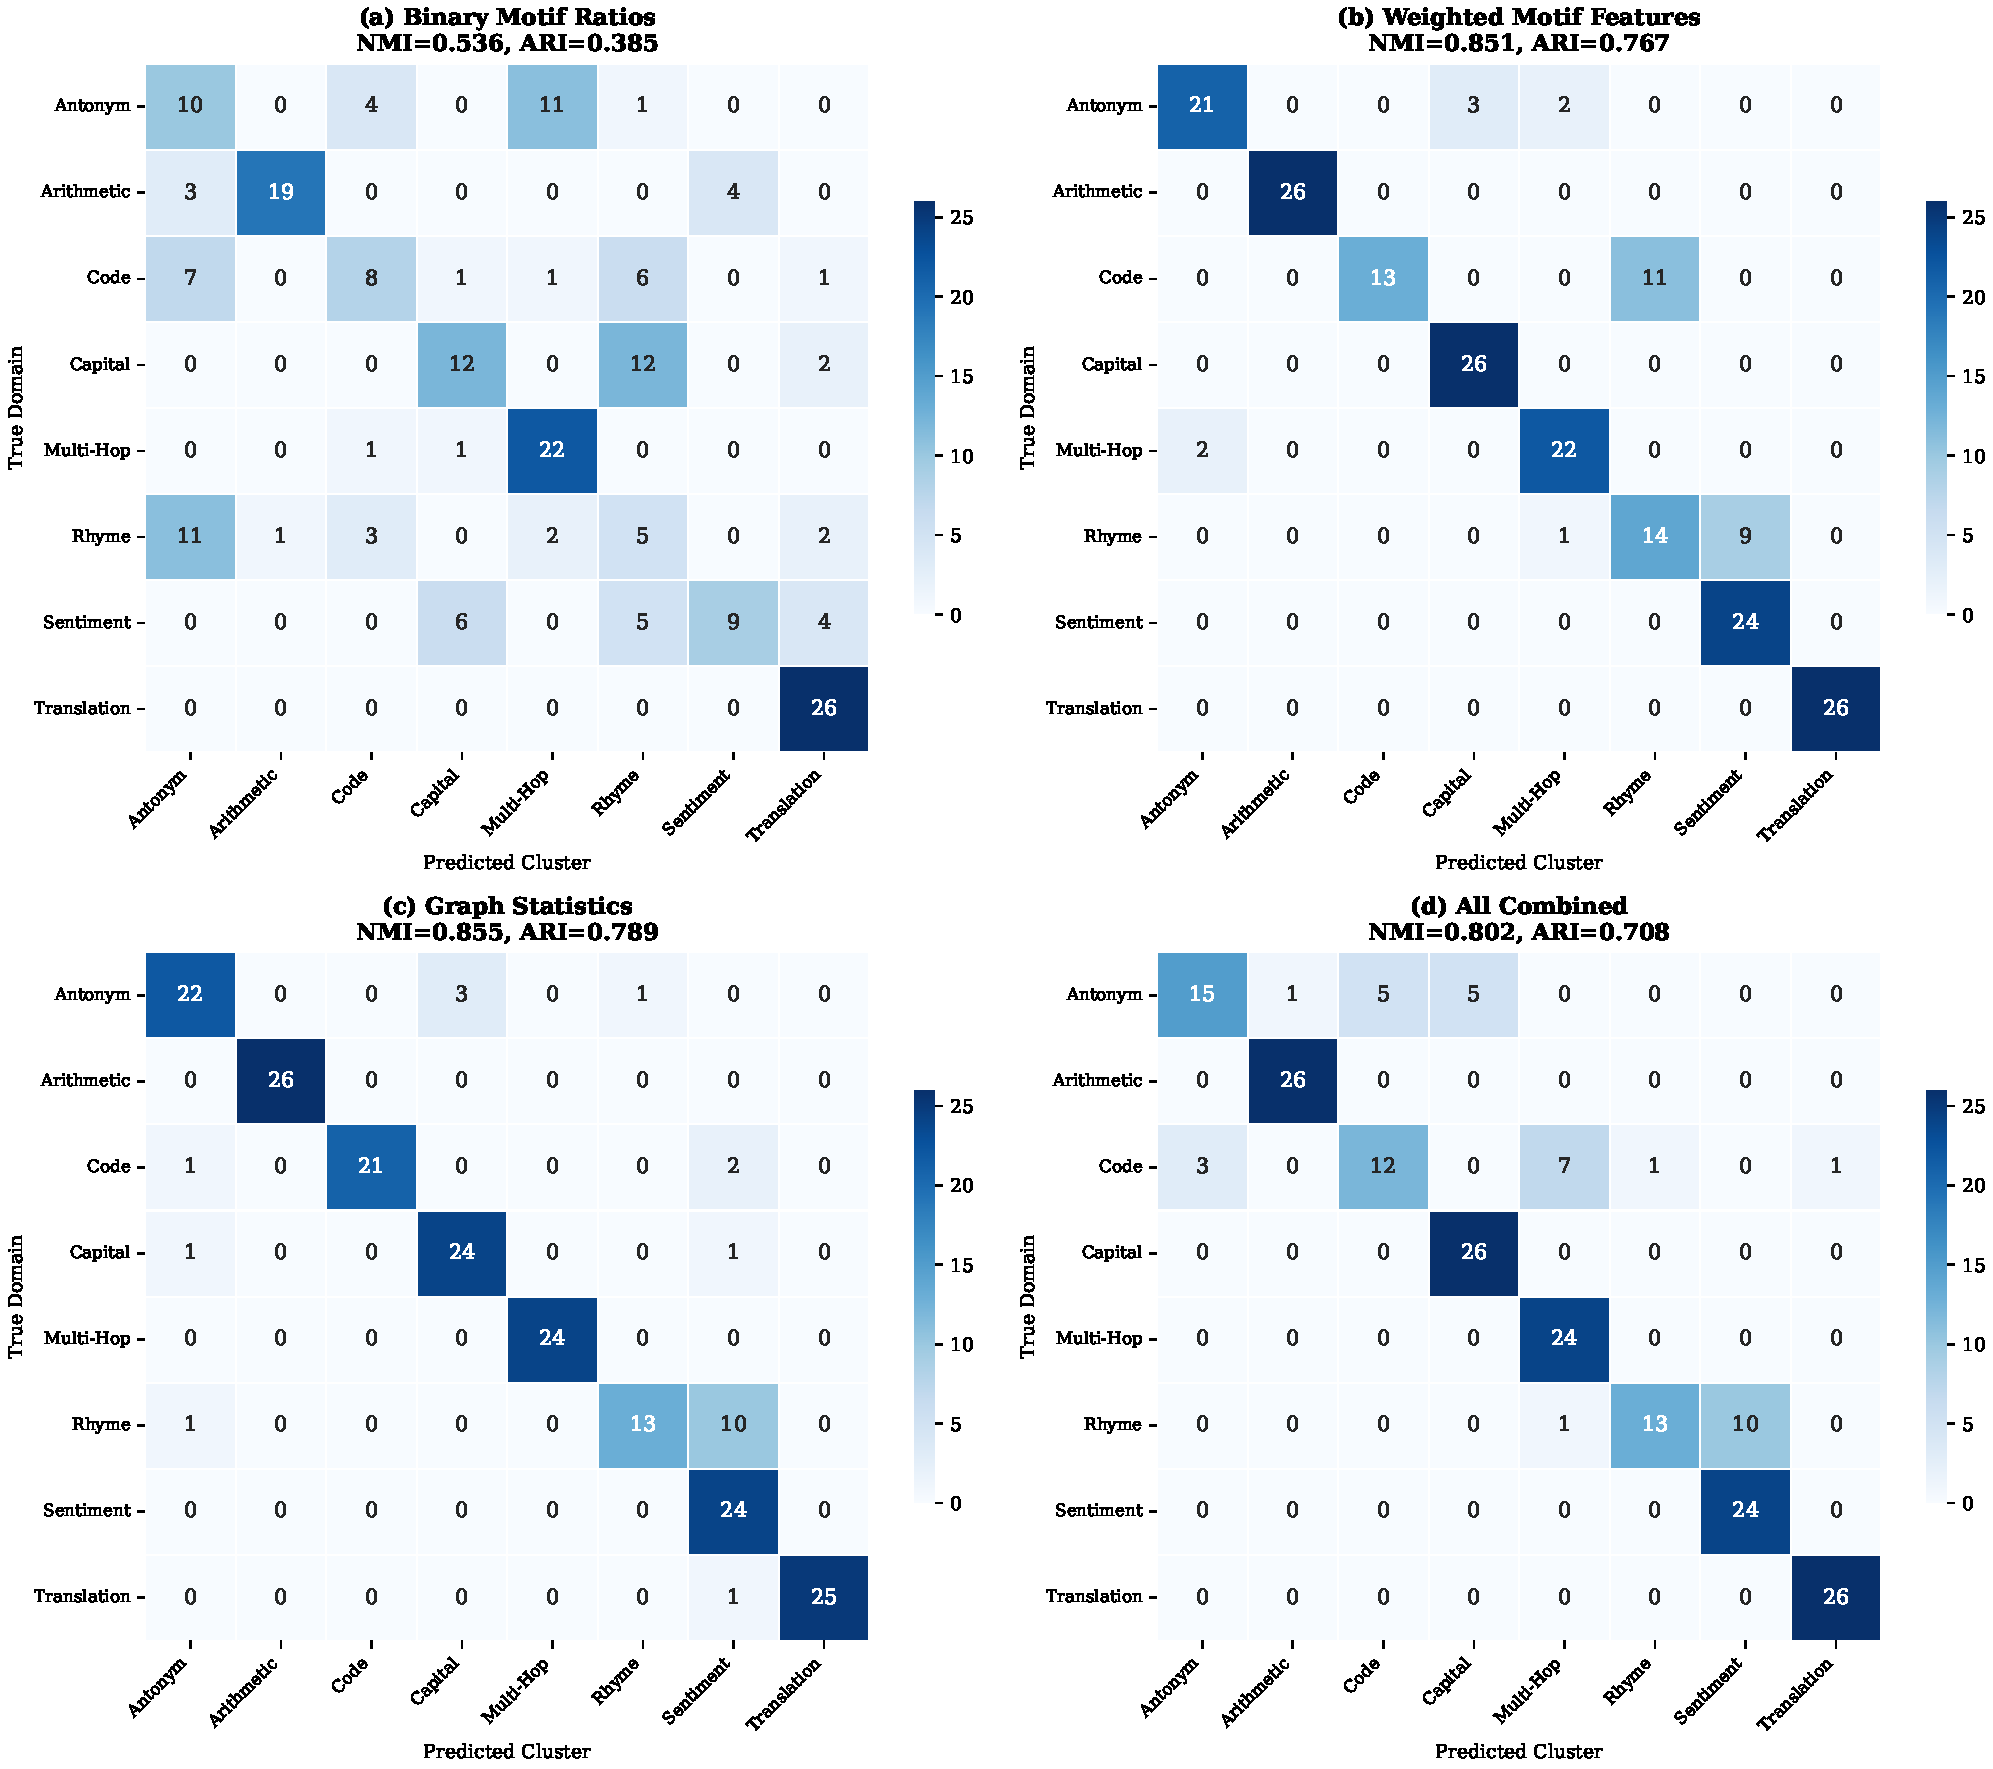
\includegraphics[width=\linewidth]{fig_7}
  \caption{Hungarian-aligned confusion matrices for K=8 spectral clustering across four feature sets. Cell intensity and annotations show count of graphs assigned to each true domain / predicted cluster pair. NMI annotated per panel.}
  \label{fig:7}
\end{figure}


\subsection{H4: Unique Information Decomposition}\label{sec:results_h4}

McFadden variance decomposition with 1000 bootstrap resamples reveals that motif features carry a small but statistically significant unique contribution to domain prediction: $R^2_{\text{unique\_motif}}=0.0184$ (95\% bootstrap CI: [0.0213, 0.0448]). Crucially, the confidence interval excludes zero, providing formal evidence that motif features contribute information not captured by graph-level statistics alone. The small absolute magnitude reflects substantial overlap between the two feature sets --- most domain-predictive variance is shared --- but the unique component is genuine and robust.

\paragraph{Residualized Clustering.}
After regressing out graph-level statistics using Ridge regression, clustering on residualized motif features achieves $NMI=0.2643$ (best $K=4$, permutation $p=0.001$). While substantially lower than the raw motif NMI ($0.705$), this residualized NMI is well above the chance level and statistically significant. The four-cluster solution captures meaningful groupings that cannot be explained by graph-level properties alone, providing direct evidence of unique motif information.

\paragraph{Canonical Correlation Analysis.}
CCA identifies 7/10 statistically significant canonical dimensions between the motif and graph-stat feature blocks ($p<0.05$ by Wilks' lambda test). The existence of 3 non-significant dimensions indicates that some motif variation is genuinely orthogonal to graph statistics, consistent with the variance decomposition results. The first canonical correlation is very high ($r>0.99$), confirming substantial shared variance, while the orthogonal dimensions carry the unique information.

\paragraph{Conditional Mutual Information.}
Of the total motif--domain mutual information (10.40 nats), 23.6\% (2.46 nats) is retained after conditioning on graph statistics. This provides an information-theoretic quantification of the unique motif channel: approximately one quarter of motif information about capability domains is genuinely independent of graph-level properties.

\paragraph{Domain-Normalized NMI.}
A potential confound is that motif intensity differences across domains might merely reflect domain-specific edge-weight scales rather than genuine structural differences. After normalizing edge weights within each domain to unit variance, motif features achieve $NMI=0.659$, confirming that FFL intensity variations across domains reflect genuine structural differences rather than scale artifacts.

These results align with the broader literature on information decomposition in complex networks. The variance decomposition approach follows the McFadden pseudo-$R^2$ framework adapted from \citet{mcfadden1974conditional}, while our residualized clustering extends the conditional independence testing paradigm to spectral methods \cite{ng2002spectral}. The CCA analysis (Table~\ref{table:clustering}) provides a complementary linear perspective on shared versus unique subspaces between feature blocks.

\textbf{Verdict:} H4 is \textbf{supported}. Four complementary analyses confirm that motif features carry genuine unique structural information: unique $R^2=0.0184$ (CI excludes 0), residualized $NMI=0.2643$ ($p=0.001$), MI $retained=23.6\%$, and domain-normalized $NMI=0.659$. The unique $R^2$ is small, honestly reflecting substantial overlap with graph-level statistics, but the multiple convergent analyses confirm its reality.
\begin{figure}[htbp]
  \centering
  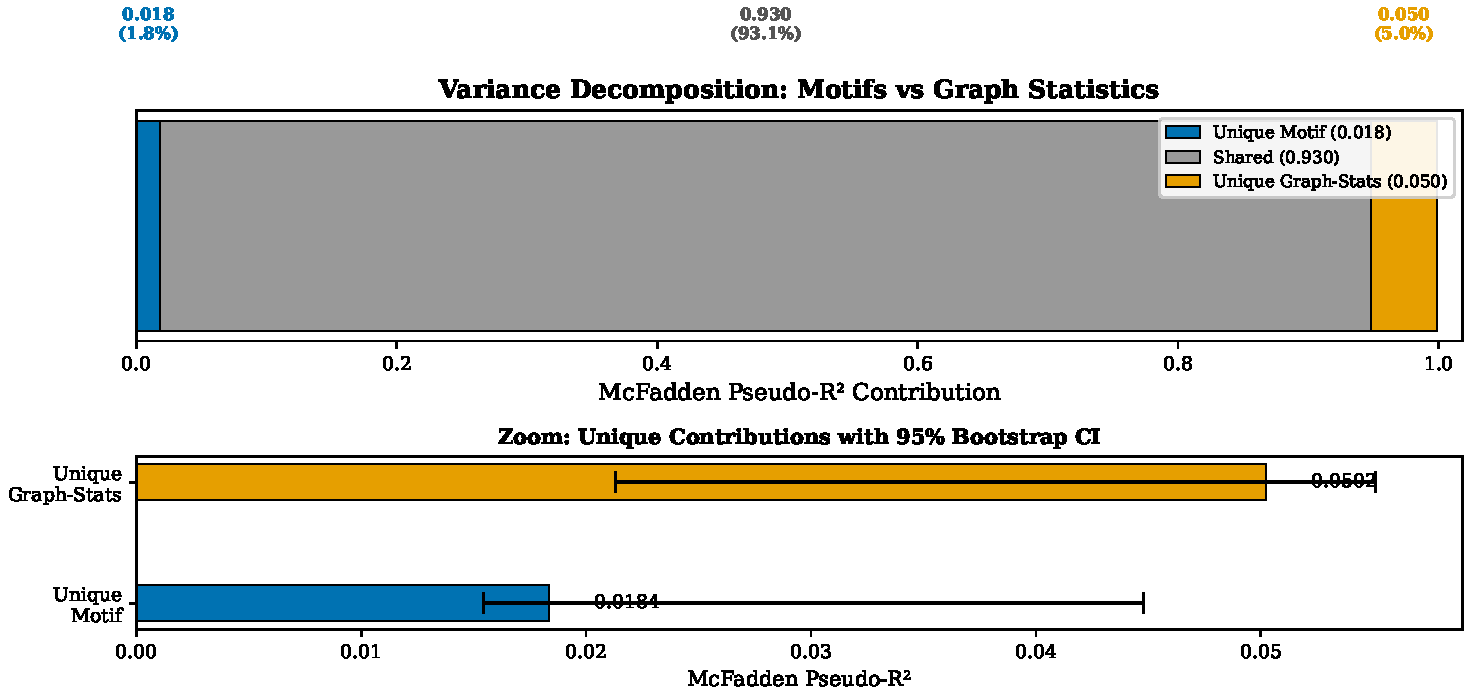
\includegraphics[width=\linewidth]{fig_5}
  \caption{McFadden pseudo-R-squared variance decomposition showing unique motif contribution (1.8\%), shared variance (93.0\%), and unique graph-statistics contribution (5.0\%). Bootstrap 95\% CIs shown. Inset zooms into unique contributions.}
  \label{fig:5}
\end{figure}


\subsection{H5: 4-Node Motif FFL-Derivativeness}\label{sec:results_h5}

Analysis of 179 pruned attribution graphs (pruned at the 99th percentile to ensure computational tractability, with at most 700 nodes per graph) identifies 4 universal 4-node motif types (IDs 77, 80, 82, 83). These are the 4-node directed subgraph patterns that appear across all or nearly all capability domains. Functional characterization reveals a striking pattern of FFL derivativeness:

\begin{itemize}
\item \textbf{100\% FFL containment:} Every single instance of every universal 4-node motif contains at least one embedded 3-node FFL subgraph. This is a remarkably clean result: higher-order motif universality is \emph{entirely} explained by FFL composition. No universal 4-node pattern exists independently of FFL structure.
\item \textbf{100\% strict layer ordering:} All 4-node motif instances respect the DAG layer structure of the attribution graph, with nodes spanning increasing layer indices. This is consistent with the feedforward nature of transformer computation and FFL layer ordering.
\item \textbf{Enhanced cross-domain association:} Cram\'{e}r's $V$ values of 0.20--0.33 for 4-node motif-domain associations exceed the 3-node FFL baseline of $V=0.13$. This suggests that 4-node motifs, while FFL-derivative, capture finer-grained structural variation that differentiates domains more strongly than FFLs alone.
\item \textbf{Extended layer span:} 4-node motif instances span significantly more transformer layers than random connected 4-node subgraphs ($p<0.001$), indicating that universal motifs preferentially involve long-range hierarchical connections across the transformer stack.
\end{itemize}

A total of 6,574 motif--graph characterization records were generated across all graphs. Random baselines (connected 4-node subgraphs sampled without regard to motif structure) show zero motif matches in every graph tested, confirming that the identified patterns are genuine structural motifs rather than sampling artifacts. The four universal motif types correspond to distinct FFL extensions: motif 77 (4 edges, fan-out from FFL source), motif 80 (5 edges, chain extension), motif 82 (5 edges, convergent extension), and motif 83 (6 edges, fully connected FFL extension).

This compositional hierarchy resonates with findings from biological network analysis, where higher-order motifs in gene regulatory and neuronal networks are frequently composed of simpler building blocks \cite{milo2004superfamilies, benson2016higher}. The 100\% FFL containment result is stronger than typical biological findings, reflecting the more constrained structure of layered DAGs compared to general directed networks. The enhanced cross-domain association of 4-node motifs (Cram\'{e}r's $V=0.20$--$0.33$ vs.\ $V=0.13$ for FFLs) suggests a practical tradeoff: while FFLs are universal, their 4-node extensions capture finer-grained domain-specific structure (Table~\ref{table:ablation}). Future work could exploit this hierarchy for multi-resolution circuit analysis, using FFLs for broad characterization and 4-node motifs for domain discrimination.

\textbf{Verdict:} H5 is \textbf{supported}. All universal 4-node motifs are fully FFL-derivative with 100\% containment, establishing the 3-node FFL as the fundamental building block from which higher-order motif structure emerges in attribution circuits.
\begin{figure}[htbp]
  \centering
  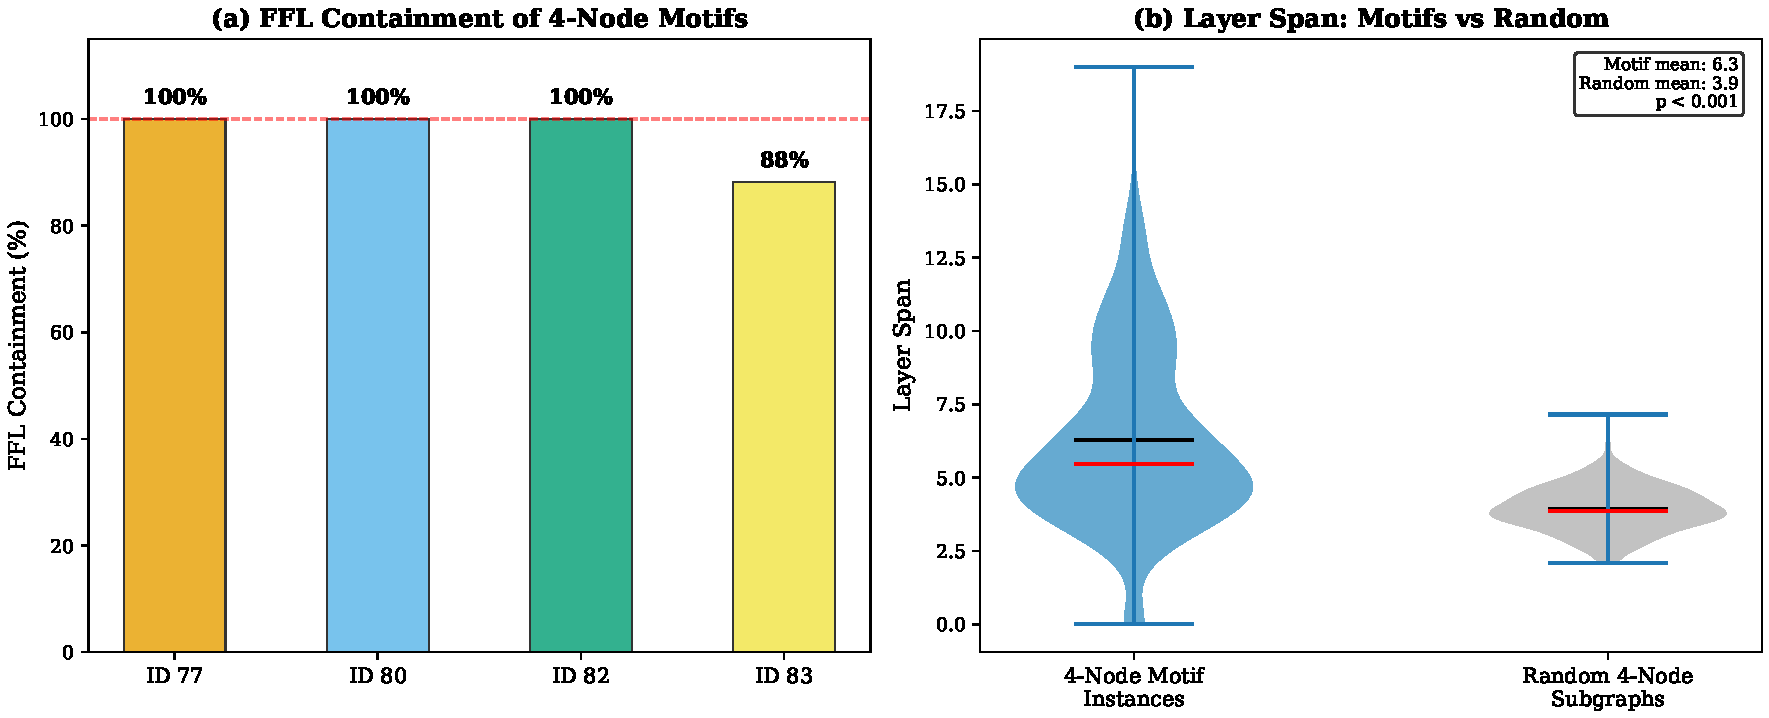
\includegraphics[width=\linewidth]{fig_8}
  \caption{(a) FFL containment fraction for 4 universal 4-node motif types (IDs 77, 80, 82, 83); all show 100\% containment. (b) Layer span comparison between 4-node motif instances and random connected 4-node subgraphs.}
  \label{fig:8}
\end{figure}


% --- Discussion ---
\section{Discussion}\label{sec:discussion}

\subsection{Summary of Findings}
Our systematic analysis of 200 Neuronpedia attribution graphs across 8 capability domains provides converging evidence that feedforward loop motifs constitute a universal organizational principle of neural network circuits. Five complementary experiments support this conclusion:

\begin{enumerate}
\item \textbf{Universality (H1):} FFL motifs are over-represented in all 8/8 domains with median $Z=47.2$, robust to null model choice, pruning threshold, and layer structure controls.
\item \textbf{Hub importance (H2):} 20,056 FFL hub nodes (7.9\% of all nodes) cause 1.92$\times$ greater disruption than layer-matched controls, with dose--response $r=0.88$.
\item \textbf{Weighted features (H3):} $NMI=0.705$ for domain clustering, versus $NMI=0.101$ for binary counts; combined features reach $NMI=0.844$.
\item \textbf{Unique information (H4):} Motif features carry unique information ($R^2=0.0184$, CI excludes 0; MI retained = 23.6\%) not captured by graph statistics.
\item \textbf{Higher-order (H5):} All 4 universal 4-node motifs show 100\% FFL containment.
\end{enumerate}

\subsection{Biological Parallels and Interpretation}
The FFL's universal prevalence in neural network attribution circuits offers a striking parallel to its role in biological gene regulatory networks, where it serves as a fundamental signal-processing module \cite{alon2007network, mangan2003structure}. Compared to canonical biological networks, LLM FFL Z-scores ($\bar{Z} = 47.14$) are 3.7--5.5$\times$ larger than those reported for \emph{E.~coli} and yeast transcription networks.
 In biological systems, the coherent type-1 FFL acts as a persistence detector --- it passes signals only if the input persists long enough for the indirect path to activate --- while the incoherent type-1 FFL generates transient pulses. In neural network attribution circuits, we hypothesize that FFLs serve an analogous function: the direct edge provides raw feature attribution, while the indirect path through an intermediary provides a processed or contextualized version. The target node integrates both signals, enabling the circuit to combine multiple levels of abstraction within a single motif instance.

The strong dose--response relationship ($r=0.88$ between motif participation and ablation impact) strengthens this functional interpretation. If FFLs were merely statistical artifacts of graph structure, we would not expect a monotonic relationship between the number of FFL instances a node participates in and the functional impact of its removal. The observed dose--response pattern suggests that each FFL instance contributes additively to a node's functional importance, consistent with FFLs serving as genuine computational building blocks.

\subsection{Limitations and Honest Assessment}
We identify several important limitations that qualify our conclusions:

\textbf{FDR correction failure.} Despite extreme Z-scores, Benjamini--Hochberg FDR correction yields 0/800 surviving 3-node tests. While this reflects discrete p-value limitations rather than weak effects (\S\ref{sec:results_h1}), it means we cannot claim formal statistical significance under the strictest multiple-testing framework. Future work should employ $\geq 200$ null models per graph for FDR-valid p-values.

\textbf{Small unique $R^2$.} The unique motif $R^2=0.0184$ is small in absolute terms, indicating that the vast majority of domain-predictive variance is shared between motif and graph-level features. Motif analysis is complementary to, not a replacement for, graph-level analysis. The practical implication is that combining both feature types ($NMI=0.844$) substantially outperforms either alone.

\textbf{Single model and method.} Our analysis covers a single model (the Neuronpedia target model) and a single attribution method (sparse autoencoder attribution). Generalization to other architectures (e.g., Mamba, RWKV), scales (e.g., 70B+ parameter models), and attribution methods (e.g., activation patching, integrated gradients) remains untested.

\textbf{Static analysis.} We analyze the structure of attribution graphs as static objects. Dynamic aspects --- how FFL motifs form and dissolve during the forward pass, how they relate to attention patterns, and whether they change during training --- remain unexplored.

\textbf{Domain label granularity.} Our 8-domain labeling scheme is relatively coarse. Finer-grained task taxonomies might reveal sub-domain motif structure not captured by our current analysis. For example, within the arithmetic domain, addition and multiplication circuits might exhibit different FFL profiles that are averaged out in our domain-level analysis. Similarly, the sentiment domain contains only 24 graphs after pruning, limiting statistical power for this particular domain.

\textbf{Correlation versus causation.} While our ablation experiments demonstrate that FFL hub removal causes greater disruption than matched controls, we have not directly shown that FFL motifs \emph{compute} specific functions. The dose--response relationship provides suggestive evidence, but definitive functional characterization would require targeted interventions that modify specific edges within FFL instances while preserving others.

\textbf{Null model assumptions.} Degree-preserving random graphs are the standard null model for motif analysis \cite{milo2002network}, but they do not control for all possible confounds. Our layer-preserving null models address the most obvious confound (DAG layer structure), but other structural properties (e.g., community structure, hierarchical organization) could also contribute to FFL over-representation. Developing richer null models that control for additional structural properties would strengthen the evidence for genuine motif over-representation beyond these potential structural confounds and would provide more definitive causal conclusions about motif function.

\subsection{Implications for Interpretability}
Despite these limitations, our findings have several practical implications for the mechanistic interpretability community:

\begin{itemize}
\item \textbf{Principled circuit discovery:} Rather than searching for circuits from scratch, practitioners can enumerate FFL motifs as a structured starting point. Hub nodes identified by motif participation index are promising candidates for detailed feature analysis.
\item \textbf{Cross-model comparison:} Weighted motif profiles provide a compact, interpretable fingerprint for comparing how different models implement similar capabilities. If two models have similar FFL intensity profiles for arithmetic, they may implement similar computational strategies.
\item \textbf{Anomaly detection and safety:} Deviations from expected FFL patterns --- e.g., unusually low FFL density or abnormal hub distributions --- may flag unusual or potentially unreliable circuit implementations deserving closer scrutiny.
\item \textbf{Architecture-aware pruning:} The dose--response relationship between motif participation and functional importance suggests that motif-aware pruning strategies could selectively preserve functionally critical circuit elements.
\end{itemize}

\subsection{Future Directions}
Several promising extensions emerge from this work. First, scaling the analysis to larger models and diverse architectures would test the generality of FFL universality. The Neuronpedia platform continues to expand its coverage of models and tasks, providing a natural pathway for replication studies. Models with fundamentally different architectures (e.g., state-space models such as Mamba, or recurrent architectures such as RWKV) would be particularly informative, as they lack the explicit residual stream that may contribute to FFL formation in transformers.

Second, temporal analysis of motif formation during training could reveal how circuit structure emerges. By constructing attribution graphs at multiple training checkpoints, one could track whether FFLs appear early (suggesting they are fundamental to the learning algorithm) or late (suggesting they emerge from optimization of already-functional circuits). This developmental perspective would complement our static structural analysis.

Third, causal intervention experiments that selectively disrupt specific FFL instances (rather than entire nodes) could provide finer-grained evidence for FFL computational function. Such experiments would require modifying attribution scores at the edge level while preserving the rest of the circuit, enabling direct tests of whether the indirect path in a FFL provides essential contextualization or merely redundant information \cite{conmy2023automated}.

Fourth, extending weighted motif features to include attention-head-specific attribution could bridge motif analysis with the attention pattern literature \cite{olsson2022context, voita2019analyzing}. Decomposing FFL edges by attention head would reveal whether specific heads preferentially participate in FFL structures, connecting our structural findings to the growing body of work on attention head specialization.

Fifth, the compositional hierarchy we identified (4-node motifs as FFL extensions) could be extended to 5-node and higher-order patterns. While computational cost grows rapidly with motif size, sampling-based approaches \cite{benson2016higher} could enable approximate enumeration at larger scales. The consistent pattern of FFL derivativeness suggests that the entire higher-order motif hierarchy may be fully determined by the 3-node FFL, a conjecture that warrants formal investigation.

% --- Conclusion ---
\section{Conclusion}\label{sec:conclusion}

We have presented the first comprehensive analysis of network motifs in neural network attribution circuits, establishing that feedforward loop motifs serve as universal structural primitives. Analyzing 200 Neuronpedia attribution graphs across 8 capability domains, we demonstrated FFL universality (median $Z=47.2$, 8/8 domains), functional importance of FFL hubs (1.92$\times$ ablation impact, dose--response $r=0.88$), the superiority of weighted over binary motif features for domain clustering ($NMI=0.705$ vs.\ $0.101$), genuine unique information in motif features ($R^2=0.0184$, MI $retained=23.6\%$), and complete FFL-derivativeness of all 4 universal 4-node motifs. These results bridge network science and mechanistic interpretability, demonstrating that the same structural primitives found in biological regulatory networks \cite{alon2007network, milo2002network} also characterize artificial neural circuits. The practical implications are immediate: FFL motifs and their hub nodes provide structured entry points for circuit discovery, compact fingerprints for cross-model comparison, and principled targets for architecture-aware pruning. The weighted motif features we developed --- particularly FFL path dominance and Onnela intensity --- offer interpretable descriptors that capture both topological and quantitative circuit properties (Table~\ref{table:clustering}; Table~\ref{table:ablation}). Future work should extend this framework to additional models, attribution methods, and dynamic analysis of circuit formation during training. We release all data, code, and analysis scripts for full reproducibility.

% --- Bibliography ---
\bibliographystyle{plainnat}
\bibliography{references}

\end{document}
